%% 
%% Copyright 2019-2020 Elsevier Ltd
%% 
%% This file is part of the 'CAS Bundle'.
%% --------------------------------------
%% 
%% It may be distributed under the conditions of the LaTeX Project Public
%% License, either version 1.2 of this license or (at your option) any
%% later version.  The latest version of this license is in
%%    http://www.latex-project.org/lppl.txt
%% and version 1.2 or later is part of all distributions of LaTeX
%% version 1999/12/01 or later.
%% 
%% The list of all files belonging to the 'CAS Bundle' is
%% given in the file `manifest.txt'.
%% 
%% Template article for cas-dc documentclass for 
%% double column output.

%\documentclass[a4paper,fleqn,longmktitle]{cas-dc}
\documentclass[a4paper,fleqn]{cas-sc}

%\usepackage[authoryear,longnamesfirst]{natbib}
%\usepackage[authoryear]{natbib}
\usepackage[numbers]{natbib}

%%%Author definitions
\def\tsc#1{\csdef{#1}{\textsc{\lowercase{#1}}\xspace}}
\tsc{WGM}
\tsc{QE}
\tsc{EP}
\tsc{PMS}
\tsc{BEC}
\tsc{DE}
%%%
% -------------------------------------------------------------------
% Pacotes para inserção de figuras e subfiguras
\usepackage{subfig,epsfig,tikz,float}		            % Packages de figuras. 
\usepackage{graphicx}
\usepackage{hyperref}
\graphicspath{ {./figs/} }
% -------------------------------------------------------------------
% \usepackage{amssymb}
% -------------------------------------------------------------------
% Pacotes para inserção de tabelas
\usepackage{booktabs,multicol,multirow,tabularx,array}          % Packages para tabela
\usepackage{natbib}
\usepackage{pifont}
\usepackage{xcolor}
% -------------------------------------------------------------------
\usepackage[utf8]{inputenc} % The default since 2018
\DeclareUnicodeCharacter{200B}{{\hskip 0pt}}
% -------------------------------------------------------------------
\begin{document}
\let\WriteBookmarks\relax
\def\floatpagepagefraction{1}
\def\textpagefraction{.001}
\shorttitle{Decentralized File Exchange Hub}
\shortauthors{Pereira Rafael et~al.}


\title [mode = title]{Decentralized File Exchange Hub: A Cloud-Native Approach}                     

\credit{Conceptualization of this study, Methodology, Software}

\author[1]{Rafael Pereira}[type=editor,
                        %auid=000,bioid=1,
                        linkedin=rafaelmendespereira,
                        orcid=0000-0001-8313-7253]
%\cormark[1]
%\fnmark[1]
\ead{rafael.m.pereira@ipleiria.pt}
   
\address[1]{Computer Science and Communications Research Centre, School of Technology and Management, Polytechnic of Leiria, 2411-901 Leiria, Portugal}

\begin{abstract}

The exchange of files has been a fundamental aspect of communication and collaboration throughout the history of computing. From the early days of floppy disks and bulletin board systems to the rise of email attachments and file-sharing platforms, the need to transfer digital files has continued to evolve. In recent years, with the proliferation of cloud-based services and an increasing focus on decentralization, the landscape of file exchange has become more complex and diverse.

In this context, our decentralized file exchange hub aims to revolutionize the way individuals and organizations share and manage files. By leveraging the power of cloud-native technologies and a modular, microservices-based architecture, our system simplifies the file exchange process, providing an intuitive and efficient experience for users. By combining the benefits of a React-based Presentation Provider served by Nginx, an Express File Management Service, a real-time Asynchronous Message Communication Server using Socket.IO, a File Gateway Service, and MongoDB Atlas as the primary database, we can offer a robust and scalable solution that adapts to the ever-changing demands of the digital world. Our system is designed to store files locally in the developer environment and Google Cloud Storage bucket for the cloud environment. The Presentation Provider service is mapped to an owned domain, \url{filexchangehub.com}.

With our system in place, users can easily exchange files without worrying about the underlying infrastructure, ensuring that they can focus on their core tasks and projects. Our cloud deployment pipeline is streamlined using Google Cloud Build and Cloud Run, as well as other GCP services such as Cloud Storage Buckets and Cloud DNS, providing a seamless transition between local and cloud environments. The infrastructure and provisioning of resources for the project are managed by Terraform, with configuration files available in the modules directory for both development and cloud environments, enhancing the maintainability and ease of deployment for the entire application. As the need for secure, reliable, and efficient file-sharing solutions continues to grow, our decentralized file exchange hub stands as a testament to the potential of modern cloud computing technologies to reshape the landscape of digital collaboration.

\end{abstract}

\begin{keywords}
Decentralized platform \sep Microservices architecture \sep Google Cloud Platform \sep Continuous Integration and Deployment (CI/CD) \sep Terraform \sep Scalability and reliability
\end{keywords}


\maketitle

\section{Introduction}

The rapid growth of cloud computing and microservices has revolutionized the way applications are developed and deployed \cite{}. As a result, there is an increasing need for effective strategies to manage the complexity and scalability of these systems \cite{}. This report explores the design and provisioning of a distributed cloud-based file exchange hub that utilizes containerization, microservices, and cloud services to achieve high availability, performance, and maintainability.

The file exchange hub aims to provide an efficient platform for users to share files with others. By utilizing a decentralized approach, the hub ensures enhanced privacy and control over shared data, while also promoting better performance and availability. The system leverages the power and flexibility of modern cloud computing technologies, such as containerization, microservices, and cloud services, to deliver a streamlined and scalable solution.

The proposed solution is divided into four main modules: Presentation Provider (Nginx), API (Express), Asynchronous Message Communication server (Socket.IO), and Database (MongoDB Atlas). Each module is designed to serve a specific purpose and can scale independently to adapt to changing loads and requirements. The application also leverages Google Cloud Platform (GCP) services such as Cloud Run, Cloud Storage Bucket, and Cloud DNS for deployment, file management, and domain management. The Presentation Provider service is mapped to a custom domain, \url{filexchangehub.com}.

The report is structured as follows: Section \ref{sec:architecture} presents the architecture of the application, detailing the purpose and design of each module. Section \ref{sec:scenarios} discusses the two scenarios in which our application can be set up and run, namely the local and cloud scenarios, and outlines their respective architectures and communication patterns. Section \ref{sec:provisioning} describes the provisioning process, emphasizing the use of GCP services, Terraform, and GitHub Actions to automate and streamline the application components' deployment. Section \ref{sec:discussion} provides a comprehensive discussion of the different scenarios, and difficulties faced during provisioning, and offers recommendations for developers working on similar projects. Finally, the report concludes with a summary of the key findings and insights gained from the project.

\section{Architecture}\label{sec:architecture}

This project follows a microservices architecture, which allows for improved scalability, resilience, and maintainability. The system is divided into several main components, each responsible for a specific aspect of the application. The following list introduces the primary components and their respective responsibilities:

\begin{itemize}
\item Presentation Provider (Nginx): This component acts as the frontend server, hosting the React web application and serving static files. It is responsible for delivering the user interface to the clients and handling incoming HTTP requests.
\item API (Express File Management Service): This component is the backend server implemented using Express.js. It manages the file uploading and downloading processes, interacting with the Database and Cloud Storage Bucket to store and retrieve files.
\item Asynchronous Message Communication Server (Socket.io): This server enables real-time communication between the clients, ensuring that users in the same room receive instant updates when a new file is shared.
\item Database (MongoDB): The database stores information about the rooms, users, and file metadata, including the bucket URL and timestamp. MongoDB was chosen for its flexibility, scalability, and performance.
\item File Gateway (Express): The File Gateway service is an Express.js application designed to efficiently stream files between clients and the cloud storage service. It acts as an intermediary, managing incoming file requests and delivering the requested files to the clients.
\item Cloud Storage Bucket (Azure Blob Storage): This component stores the uploaded files, providing a reliable and scalable storage solution.
\end{itemize}

In this architecture, each component communicates with the others through well-defined interfaces, allowing for efficient collaboration and easy maintenance. The use of containerization and cloud-native deployment further enhances the system's scalability and resilience.

\subsection{Presentation Provider: Nginx-based Frontend}

The presentation layer of our file exchange hub is built using a React web application. We utilize Nginx as a reverse proxy and web server to serve the static content generated by the React application. Nginx offers excellent performance, stability, and low resource usage, making it an ideal choice for our frontend. Furthermore, its ability to handle a large number of simultaneous connections ensures a responsive user experience, even during peak loads.

\subsection{API: Express-based File Management Service}

Our file management service is implemented using Node.js with the Express framework, providing a robust and scalable API for managing file metadata and coordinating file transfers. This service is responsible for handling managing file metadata and communicating with the File Gateway service for actual file uploads and downloads. Express is chosen for its ease of use, extensive documentation, and compatibility with Node.js, which allows for efficient development and seamless integration with other components of the File Exchange Hub.

\subsection{Database: MongoDB}

MongoDB, a NoSQL database, is utilized to store information about rooms, files, and users. It's flexible schema and horizontal scalability make it a fitting choice for our cloud-native application, as it can easily adapt to changing requirements and handle large volumes of data. Additionally, MongoDB provides a rich query language and high-performance indexing capabilities, allowing for efficient data retrieval and manipulation.

\subsection{Asynchronous Message Communication Server: Socket.IO}

To enable real-time communication and notifications within our file exchange hub, we employ Socket.IO, a popular library for real-time web applications. This server facilitates instant messaging between users in the same room, ensuring a seamless and interactive experience for all participants. Socket.IO is selected for its flexibility, reliability, and compatibility with various platforms and transports, making it a powerful solution for real-time communication in our application.

\subsection{File Gateway: Express-based File Streaming Service}

The File Gateway service is built with the Express framework, chosen for its simplicity, and compatibility with Node.js. It efficiently streams files between clients and local/cloud storage service by managing incoming file requests and delivering the requested files to the clients. Express provides a robust set of features that simplify the development process and enable seamless integration with other components of the File Exchange Hub.

\subsection{Cloud Storage Bucket: Azure Blob Storage}

To store and manage the actual files exchanged by users, we leverage Azure Blob Storage. This fully managed object storage service offers high availability, durability, and scalability, allowing our file exchange hub to efficiently store, retrieve, and share files. The choice of Azure Blob Storage is driven by its integration with other Azure services, its security features, and its cost-effective pricing model, making it a suitable solution for our application's file storage needs.

\section{Scenarios} \label{sec:scenarios}

In this section, we will discuss the two scenarios in which our application can be set up and run: the local scenario and the cloud scenario. Each scenario has its own architecture and communication patterns between the different services. Understanding these scenarios helps in setting up, testing, and deploying the application effectively.

\subsection{Local scenario}

In the local scenario, all components are hosted and run locally on the developer's machine. The following diagram (Figure \ref{fig:architectureLocal}) depicts the relationships between the components:

\begin{figure}[htb]
\centering
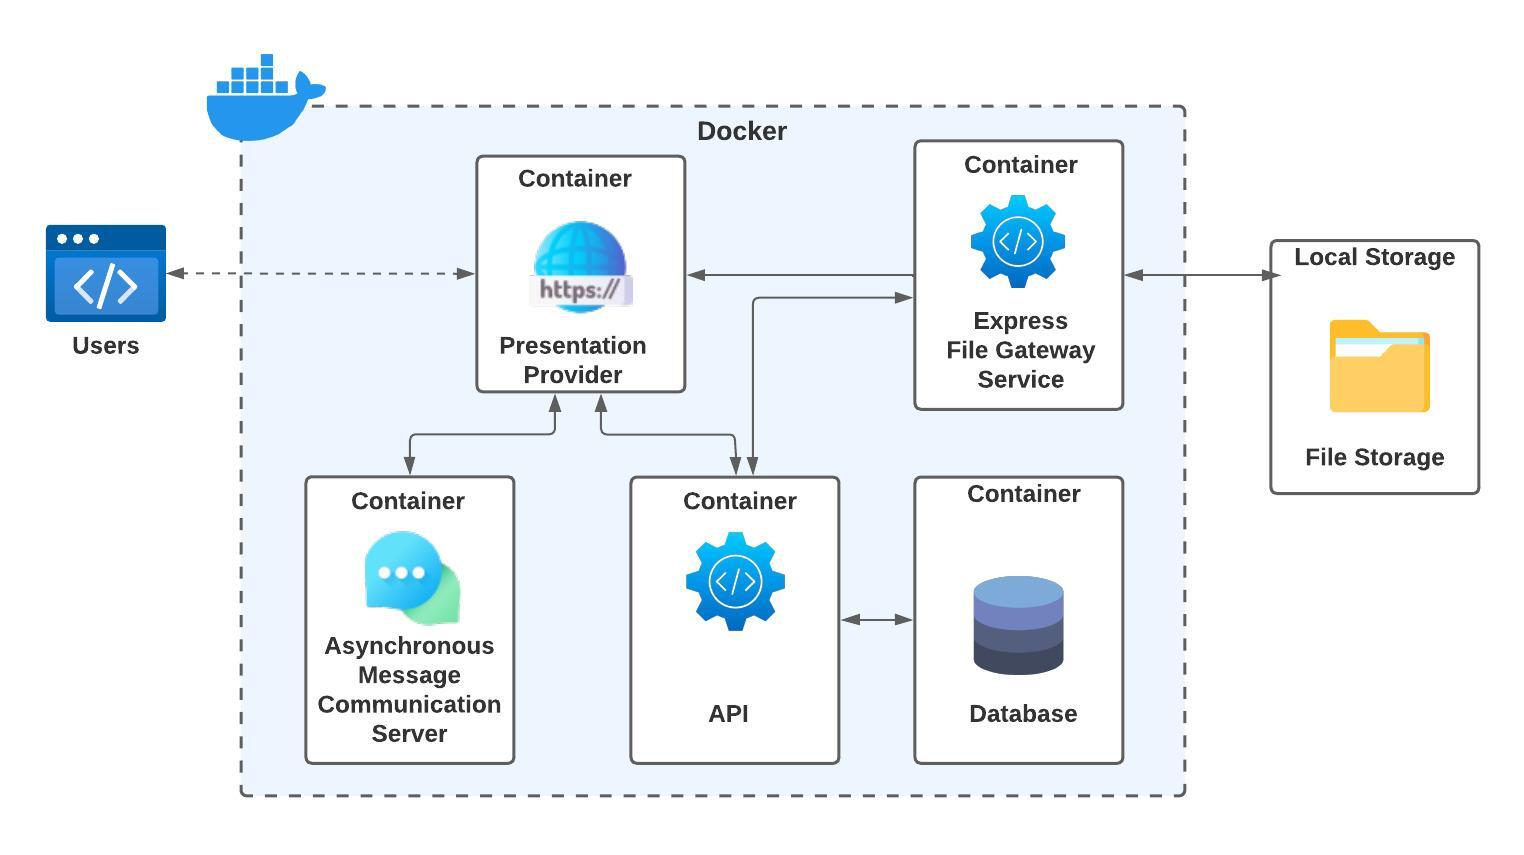
\includegraphics[width=9cm]{LocalArch.jpeg}
\caption{Local system architecture diagram.}
\label{fig:architectureLocal}
\end{figure}

In this setup, the Presentation Provider communicates directly with the Express File Management Service, Asynchronous Message Communication Server, and File Gateway Service, which are all running on the same local machine. The Express File Management Service is responsible for managing file metadata. The Asynchronous Message Communication Server handles real-time communication, and the File Gateway Service manages the actual file uploads and downloads by interacting with the local storage. Local provisioning is performed using both Docker Compose and Terraform, streamlining the process of setting up the local environment.

\subsection{Cloud scenario}
In the cloud scenario, the services are deployed on Google Cloud Run, the file storage is handled by Google Cloud Storage, and the database is deployed as a cluster on MongoDB Atlas. The following diagram (Figure \ref{fig:architectureCloud}) depicts the relationships between the components:

\begin{figure}[htb]
\centering
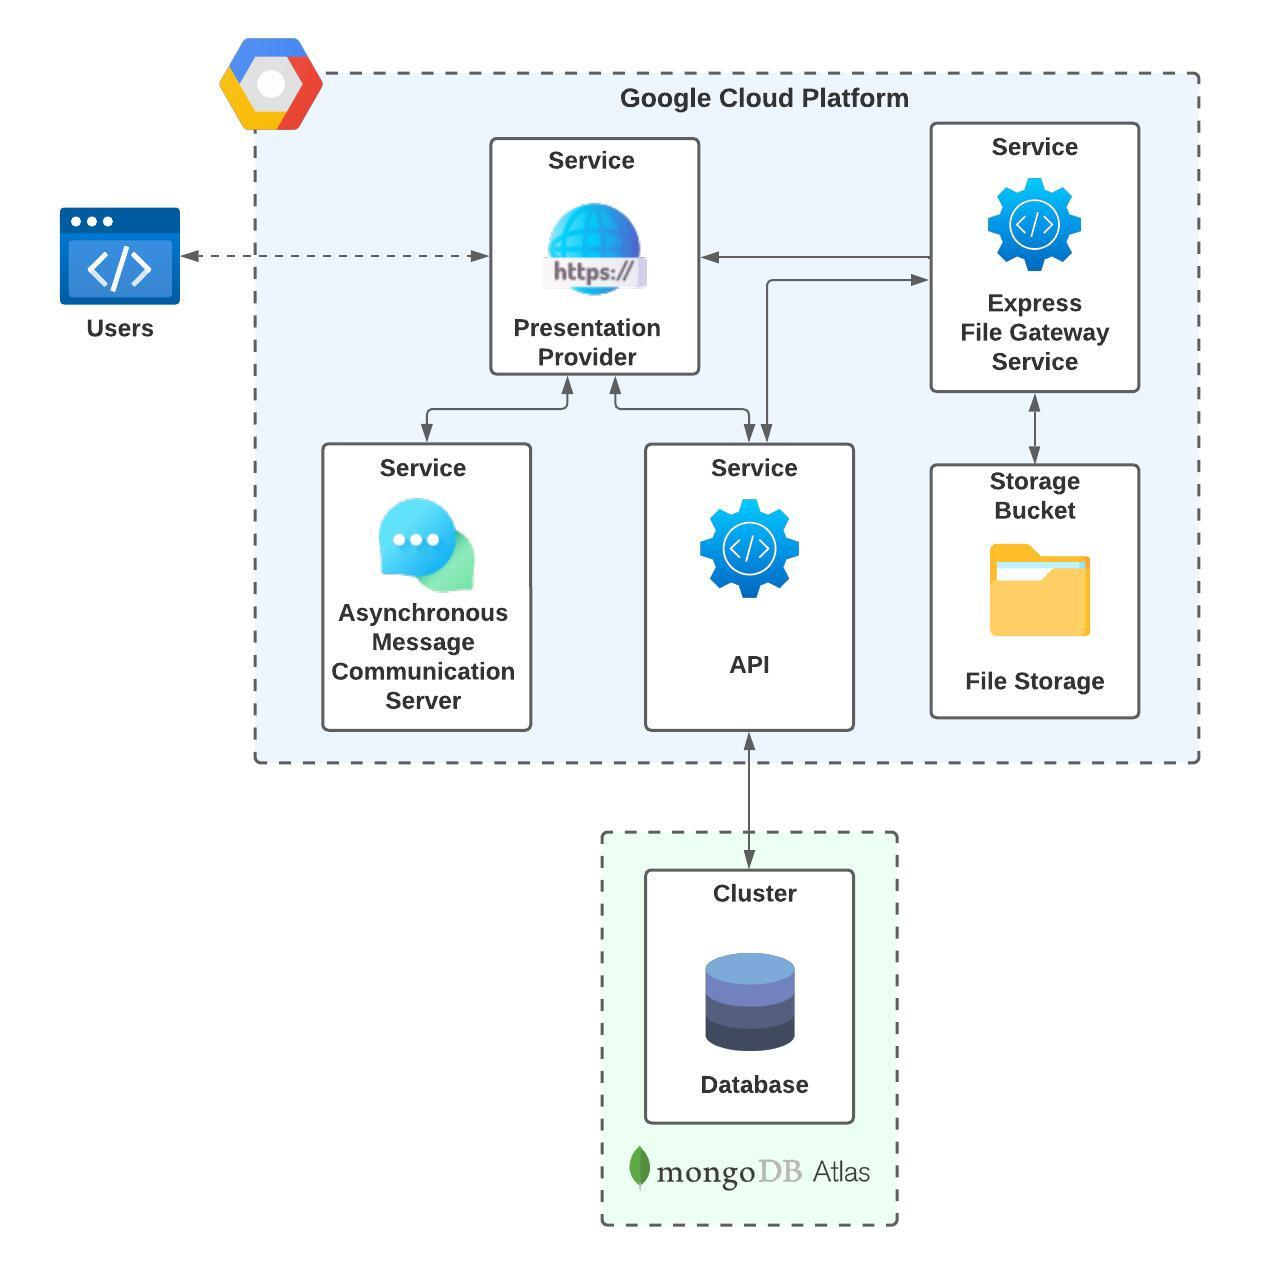
\includegraphics[width=8cm]{CloudArch.jpeg}
\caption{Cloud system architecture diagram.}
\label{fig:architectureCloud}
\end{figure}

In this setup, the Presentation Provider communicates with the Express File Management Service, Asynchronous Message Communication Server, and File Gateway Service through their respective exposed endpoints. The Presentation Provider service is mapped to an owned domain, \url{https://filexchange.com}. The Express File Management Service is responsible for managing file metadata. The Asynchronous Message Communication Server handles real-time communication, and the File Gateway Service manages the actual file uploads and downloads by interacting with Google Cloud Storage. This architecture provides better scalability and reliability, as each service can be independently managed and scaled in response to the system's demands.

The file bucket is not public; only users with access to the file download URL can access it, which happens if the URL is shared on purpose or someone has access to the Room within the File Exchange Hub platform. For privacy reasons and reduced allocated space, files inserted in the file bucket have a lifetime of 1 day, after which they are automatically deleted by the settings defined when creating the bucket. Additionally, file records in the MongoDB Atlas database have an expiration time associated with them, meaning that these expired files can no longer be consulted.

\section{Cloud Provisioning} \label{sec:provisioning}

The cloud provisioning process is designed to ensure a smooth transition from development to cloud, leveraging the power of various Google Cloud Platform (GCP) services and MongoDB Atlas. The provisioning strategy uses GCP's Cloud Run, Google Cloud Storage, Google Cloud DNS, and Cloud Build services, along with GitHub Actions, Docker Hub, and Terraform, for automating and streamlining the process. Figure \ref{fig:provisioning} presents a diagram of the provisioning process, illustrating the steps and relationships between each involved service.

\begin{itemize}
\item GitHub Actions: This service automates the build and provisioning of the application components. It is triggered by a push to the repository, builds the Docker images, and pushes them to Docker Hub.
\item Terraform: Terraform applies the infrastructure changes and triggers Cloud Run to pull Docker images from Docker Hub and deploy the containerized services, as well as create the necessary Google Cloud Storage buckets and Google Cloud DNS configurations, and configure the MongoDB Atlas cluster.
\item GCP Services and MongoDB Atlas: A combination of Google Cloud Run, Google Cloud Storage, and Google Cloud DNS services are used to deploy, store, and map the application components to the custom domain. MongoDB Atlas is used for the deployment and management of the database cluster.
\end{itemize}

Figure \ref{fig:provisioning} depicts the provisioning process and the relationships between the components, illustrating the following flow: (1) The developer commits and pushes changes to the repository, (2) which triggers GitHub Actions to (3) build and push Docker images to Docker Hub for the modified services. (4) Terraform is then initiated, applying infrastructure changes, (5) retrieving and writing the Terraform state to the cloud storage bucket as the remote backend for persistence and collaboration, (6) subsequently triggering Cloud Run, Google Cloud Storage, Google Cloud DNS, and MongoDB Atlas configurations. (7) Cloud Run pulls images from Docker Hub, (8) deploys the containerized services (Presentation Provider, API, Asynchronous (Message) Communication Server, and File Gateway), and (9) maps the Presentation Provider service to the domain \url{https://filexchange.com}.

\begin{figure}[h]
\centering
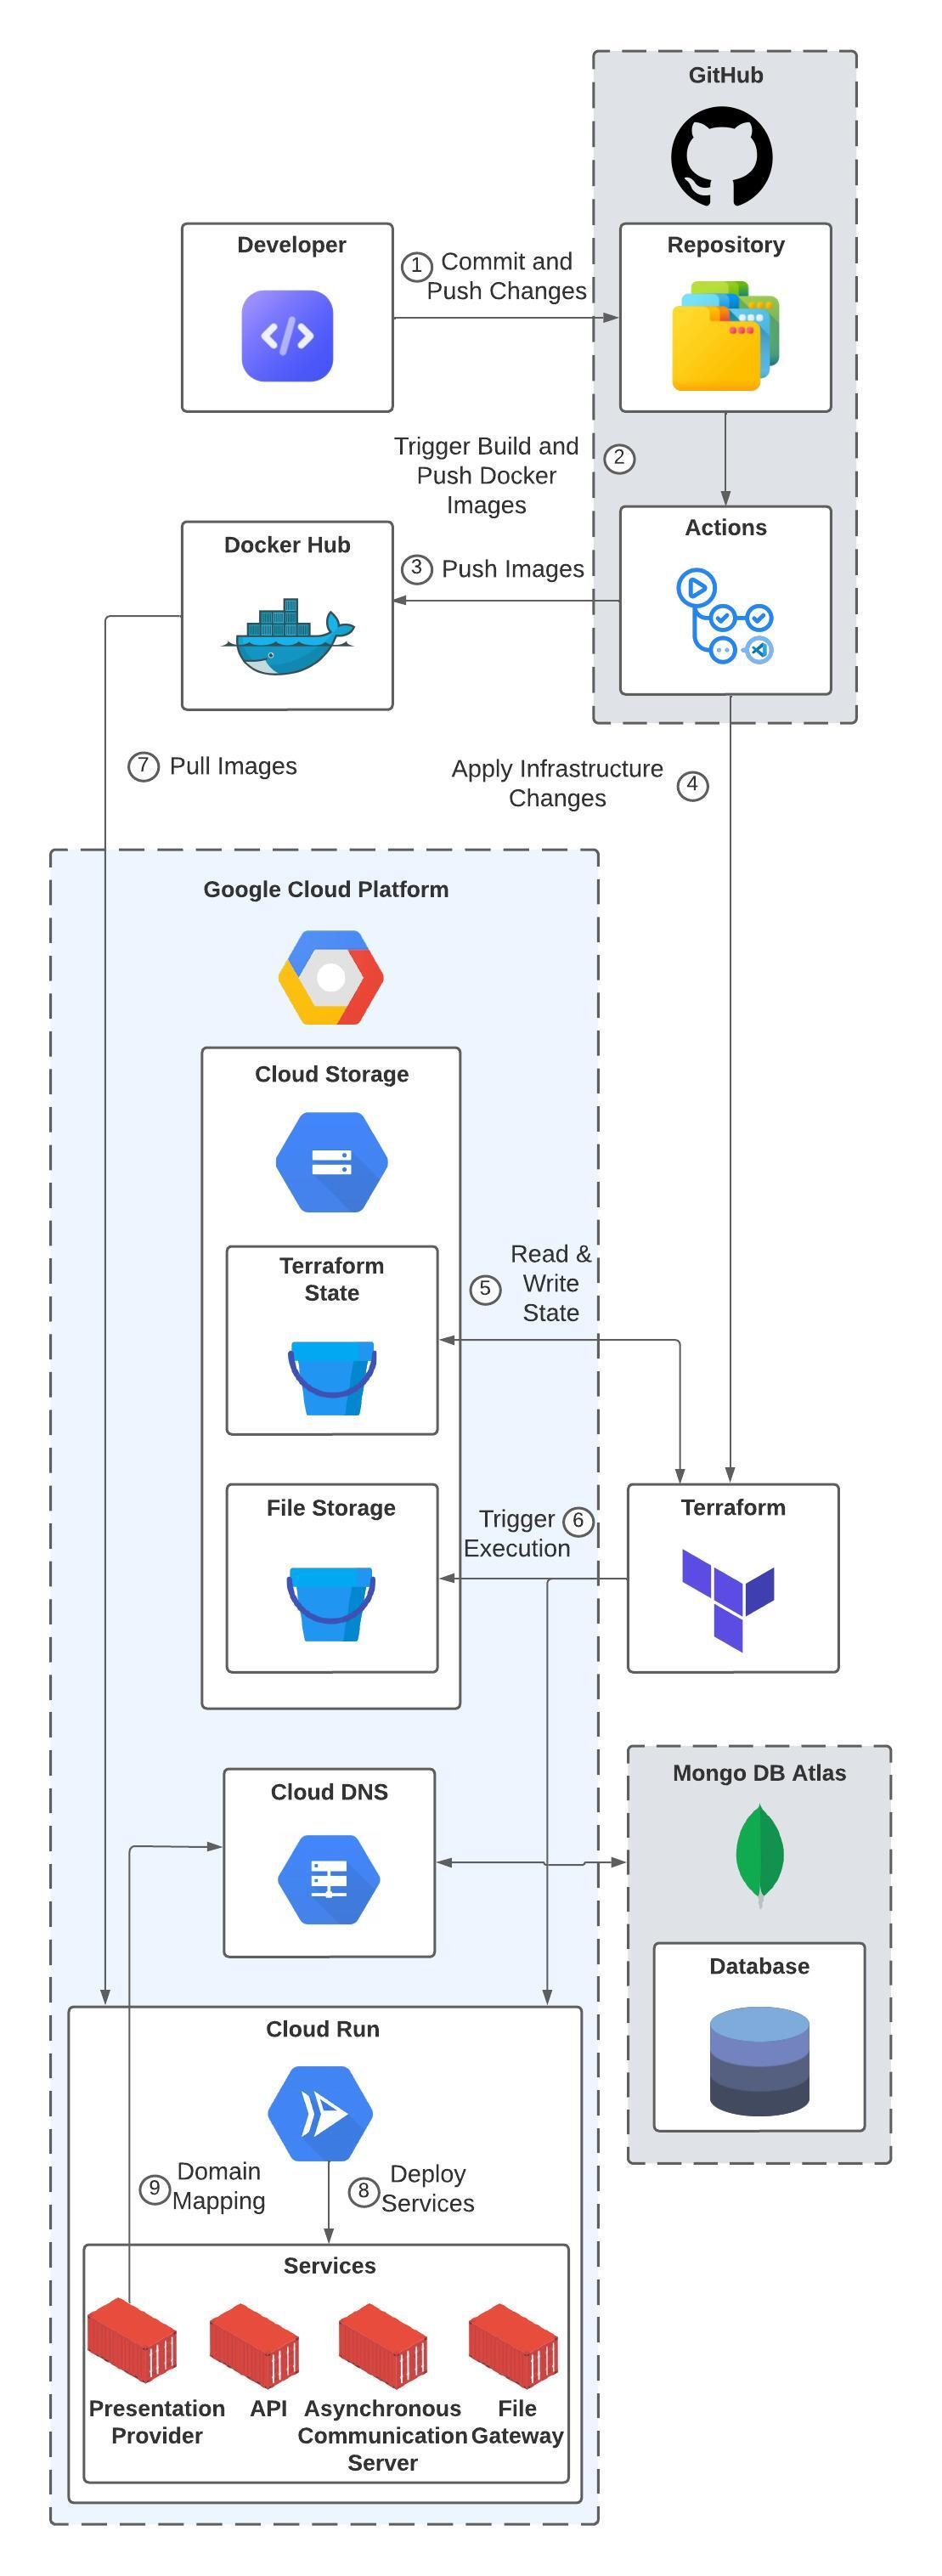
\includegraphics[width=7cm]{CloudProvisioning.jpeg}
\caption{Cloud provisioning process diagram.}
\label{fig:provisioning}
\end{figure}

The provisioning process ensures that the application components are consistently built and deployed across environments, minimizing human error and facilitating continuous integration and delivery.

\subsection{Continuous Integration and Continuous Deployment with GitHub Actions and Terraform}

To streamline the software development process and ensure a consistent and efficient release cycle, we implemented a Continuous Integration and Continuous Deployment (CI/CD) pipeline using GitHub Actions and Terraform. GitHub Actions automates the process of building and pushing Docker images to Docker Hub for each modified service, while Terraform manages the infrastructure required to deploy and update the services on Google Cloud Run, create Google Cloud Storage buckets, and configure Google Cloud DNS, as well as configuring the MongoDB Atlas cluster.

When changes are pushed to the repository, GitHub Actions analyzes the respective commits to identify which services have been modified. Based on this analysis, it triggers a separate automated workflow for each modified service. To ensure a seamless deployment process, we have implemented a mechanism within the GitHub Actions workflows to manage dependencies among the services. The dependencies can be summarized as follows: the Presentation Provider relies on both the API and Asynchronous Message Communication Server, while the API depends on the File Gateway and Database. This arrangement ensures that each service waits for its required dependencies to be available before proceeding, promoting a smooth and efficient deployment process.

To manage these dependencies, the workflows are designed to check for the availability of required components before executing further steps. This is done by periodically polling for the existence of required GitHub Variables, which indicate that the respective components have been successfully deployed.

However, having multiple workflows creates a challenge, as more than one workflow may try to access the shared Terraform state simultaneously. To address this issue, we implemented a retry mechanism that ensures that workflows wait for access to the Terraform state, preventing conflicts.

These workflows build and push the updated Docker images for the corresponding microservices to Docker Hub as part of the Continuous Integration process. Following the successful completion of this step, the workflow for each modified microservice initiates the Terraform CLI to manage the provisioning of the respective services on their providers, such as Google Cloud Run, Google Cloud Storage, Google Cloud DNS, and MongoDB Atlas, as part of the Continuous Deployment process.

Using Terraform, we define the infrastructure for each microservice as code, including Google Cloud Run services, IAM policies, Google Cloud Storage buckets, Google Cloud DNS configurations, and MongoDB Atlas cluster. This approach enables us to maintain a version-controlled and easily auditable infrastructure while also allowing for seamless updates and configuration changes. By integrating with GitHub Actions, we ensure that every push to the repository automatically triggers Continuous Integration and Continuous Deployment for the modified services, resulting in a streamlined and consistent release process.

\subsection{Google Cloud Platform and MongoDB Atlas: Scalable Cloud Services}

Google Cloud Platform (GCP) and MongoDB Atlas provide a suite of cloud services that enable developers to build, deploy, and scale applications efficiently. For this project, we leveraged several GCP services, including Google Cloud Run, Google Cloud Storage, and Google Cloud DNS, as well as MongoDB Atlas for the database cluster.

\subsubsection{Cloud Run: Scalable Containerized Services}

Google Cloud Run is a serverless platform that enables the deployment and management of containerized applications. By leveraging the power of containers, Cloud Run allows developers to focus on writing code without worrying about the underlying infrastructure. The platform automatically scales applications based on demand, ensuring optimal resource usage and minimizing costs.

\subsubsection{Google Cloud Storage: Storing Files and Terraform State}

Google Cloud Storage is a highly scalable and durable object storage service. In this project, we used Google Cloud Storage for two purposes: storing the uploaded files from users in one bucket and storing the Terraform state in another dedicated bucket. By storing the Terraform state in a cloud storage bucket, we enable team members to collaborate on infrastructure changes and maintain a persistent and version-controlled state.

\subsubsection{Google Cloud DNS: Custom Domain Configuration}

Google Cloud DNS is a high-performance, resilient, and global DNS service that enables the mapping of the Presentation Provider service to the custom domain \url{https://filexchangehub.com}. By utilizing Google Cloud DNS, we can manage DNS records programmatically using Terraform, ensuring that our domain configurations are version-controlled and easily updatable.

\subsubsection{MongoDB Atlas: Managed Database Cluster}

MongoDB Atlas is a fully managed, global, and scalable cloud database service that provides a powerful and flexible platform for deploying, managing, and scaling a MongoDB cluster. In this project, we used MongoDB Atlas to deploy and manage our database cluster, ensuring optimal performance, high availability, and seamless scalability. By configuring the MongoDB Atlas cluster through a dedicated Terraform module, we can maintain a version-controlled and easily auditable infrastructure for our database.

The combination of GCP services and MongoDB Atlas allows us to build a scalable, resilient, and efficient file exchange system that demonstrates the power and flexibility of modern cloud computing technologies for software applications.

\section{Discussion} \label{sec:discussion}

Throughout the development of our decentralized file exchange hub, we encountered various challenges and gained valuable insights into deploying applications both locally and in the cloud. In this section, we will discuss the different scenarios, difficulties faced during provisioning.

Comparing the local and cloud scenarios, we noticed that while local deployment is more straightforward to set up and manage, it lacks the scalability and reliability offered by cloud deployment. In the local scenario, all components run on the developer's machine, which simplifies communication between services but limits the system's ability to handle high loads and provide high availability. On the other hand, deploying our application to the cloud using Google Cloud Platform services, such as Cloud Run, Cloud Storage, Cloud DNS, and MongoDB Atlas, enables us to achieve better scalability and reliability while maintaining a modular architecture. This approach allows each service to be independently managed, scaled, and updated, thus improving the system's overall resilience and flexibility.

During the provisioning process, we faced several challenges, including configuring custom domain mapping, setting up Google Cloud Storage buckets for storing uploaded files and Terraform state, ensuring security across all components, managing dependencies between the GitHub Actions workflows, and addressing potential issues with concurrent Terraform executions. To overcome these challenges, we relied heavily on documentation, best practices, and online resources, which proved invaluable in guiding our development efforts.

One key decision made during the project development was to implement CI/CD using GitHub Actions and Terraform. This approach allowed us to streamline the development process and maintain a consistent release cycle while also ensuring that our infrastructure is version-controlled and easily auditable. Furthermore, we developed mechanisms to manage dependencies between services and implemented a retry strategy to handle potential conflicts in Terraform state access, which contributed to a robust and reliable deployment system.

\section{Lessons Learned and Recommendations}

Throughout the development and deployment of our decentralized file exchange hub, we gained valuable insights and learned several lessons that can be beneficial for other developers embarking on similar projects.

\begin{itemize}
	\item \textbf{Understand the trade-offs between local and cloud deployments:} It is essential to invest time in understanding the differences between local and cloud deployments and choose a deployment strategy that best aligns with your application's requirements and constraints.
	\item \textbf{Embrace modern development practices:} Adopting practices such as CI/CD, infrastructure as code, and dependency management can significantly improve the development process and overall application resilience.
	\item \textbf{Leverage documentation and online resources:} Relying on available documentation, best practices, and online resources can be invaluable in guiding your development efforts and overcoming challenges.
	\item \textbf{Test each service independently and as part of the larger system:} Thoroughly testing each service in isolation and within the context of the entire system is crucial to ensure seamless integration and functionality.
\end{itemize}

By sharing these lessons learned and recommendations, we aim to contribute to the growing body of knowledge and best practices in the field, and hope that our experiences can serve as a guide for developers embarking on similar endeavors. Ultimately, embracing modern development practices, understanding the nuances of different deployment strategies, and leveraging available resources and documentation are essential ingredients for a successful project outcome.

\section{Conclusion}

In this paper, we addressed the problem of creating a secure and scalable decentralized file exchange hub that provides a viable alternative to traditional centralized solutions. Our solution leverages the benefits of a microservices architecture, using Google Cloud Platform services and MongoDB Atlas to create a distributed and modular system that offers enhanced scalability, reliability, and flexibility compared to centralized file exchange platforms.

We implemented our solution using a variety of technologies, including Docker for containerization, GitHub Actions for CI/CD, and Terraform for infrastructure as code. Our deployment process was designed to be efficient and streamlined, automating the provisioning of resources on Google Cloud Platform and MongoDB Atlas to ensure a consistent release cycle.

Throughout the project, we encountered numerous challenges, such as managing dependencies between services, and addressing potential conflicts in Terraform state access. Through careful planning, resourceful problem-solving, and adherence to best practices, we successfully overcame these challenges and developed a robust and reliable file exchange hub.

%% Loading bibliography style file
%\bibliographystyle{model1-num-names}
%\bibliographystyle{cas-model2-names}
%\bibliographystyle{unsrt} % Estilo de Bibliografia
% Loading bibliography database
%\bibliography{cas-refs}


%\vskip3pt

\end{document}
